\documentclass[../../AdvancementSummary.tex]{subfiles}

\begin{document}





%%%%%%%%%%%%%%%%%%%%%%%%%%%%%%%%%%%%%%%%%%%%%%%%%%%
\section{Electrostatics}
%%%%%%%%%%%%%%%%%%%%%%%%%%%%%%%%%%%%%%%%%%%%%%%%%%%

\subsection{Introduction}

% some disordered proteins associate with the cell membrane
Intracellular subunits of many receptors associate with the cell membrane prior to signaling \cite{Xu2008, Shi2013, Zhang2011, Dobbins2016}. 
% then fall off upon triggering
However, several of these chains have been shown to dissociate from the membrane after the extracellular receptor receives a stimulus \cite{Zhang2011, Dobbins2016}.
% in particular, TCR zeta associates to the membrane
In particular, CD3$\zeta$ associates with the membrane, sequestering the tyrosines in the bilayer and preventing phosphorylation by Lck \cite{Aivazian2000, Zhang2011, Shi2013}.
% falls off upon triggering (if able to become phosphorylated)
Stimulating the TCR with an antigen will cause the CD3$\zeta$ chain to dissociate from the membrane \cite{Zhang2011}.
% phosphorylation prevents association
Additionally, phosphorylated CD3$\zeta$ does not associate with the membrane, but remains anchored by its transmembrane region  \cite{Aivazian2000, Zhang2011}.
% phosphorylation is required for TCR triggering to release membrane association
However, mutation of the tyrosines to phenylalanine, to prevent phosphorylation, abrogates this effect. Thus, phosphorylation is required to for $\zeta$ chain dissociation from the membrane even with TCR triggering  \cite{Zhang2011}.

% basic residue regions are important for membrane-association
Basic residue regions in the CD3$\zeta$ and $\epsilon$ chains play a major role in maintaining the association between the polymer and the membrane.
% eliminating basic residues eliminates association
Studies show that mutation of the basic residue regions is sufficient to cause the protein to dissociate from the membrane \cite{Zhang2011}.
% phosphorylation eliminates association despite basic residues
%Fully phosphorylated tyrosines are also sufficient to pull the protein away from the membrane, even when basic residue regions are present \cite{Zhang2011}.

% calcium influx also pulls chains away
TCR triggering creates a calcium influx. Calcium then interferes with the interactions of the basic residues with the membrane, causing the CD3$\zeta$ chain to dissociate from the membrane \cite{Shi2013}. Prior to the calcium influx, the $\zeta$-chain tyrosines remain sequestered in the membrane, preventing signaling. However, since TCR triggering is the causal event of T cell signaling, it is unclear how the first $\zeta$ chains dissociate from the membrane to propagate the signal. 

Close association with the membrane inhibits ligands from binding to their target site. CD3$\zeta$ tyrosines are sequestered in the membrane, preventing phosphorylation by Lck \cite{Aivazian2000, Shi2013}. Although the tyrosines will spend much of their time sequestered in the membrane, they will still transiently enter the cytoplasm. When this occurs, Lck would be able to phosphorylate the tyrosine, creating a large negative charge on the chain. This phosphotyrosine could repel the negative polar heads of the membrane, making it more favorable for that section of the polymer to pull out of the membrane. We hypothesize that entropic fluctuations of the tyrosines in and out of the membrane are sufficient to lead to an initial phosphorylation event. We also hypothesis that following this initial event, there would be a cooperative enhancement of the accessibility of neighboring tyrosines.

Here we simulate electrostatic potentials acting on the disordered chain. We first fit parameters of the potentials to match the characteristics seen experimentally, e.g. phosphorylation removes association with the membrane. We will next investigate the accessibility of each tyrosine and how this is impacted by phosphorylation of neighboring tyrosines. From this, we will determine if cooperativity or sequential binding can arise from phosphorylation under these circumstances.

%%%%%%%%%%%%%%%%%%%%%%%%%%%%%%%%%%%%%%%%%%%%%%%%%%%%%%%%%%%%%%%%%%%%%%%%%%%%%%%%%%%%%%%%%%%%%%%%%%%%%
%%%%%%%%%%%%%%%%%%%%%%%%%%%%%%%%%%%%%%%%%%%%%%%%%%%%%%%%%%%%%%%%%%%%%%%%%%%%%%%%%%%%%%%%%%%%%%%%%%%%%

\subsection{Model and Methods}


A molecular dynamics simulation of CD3$\epsilon$ indicates an approximately Gaussian distribution of the tyrosines, centered at the phospholipid heads of the membrane \cite{Lopez2015}.

We model the polymer-membrane association as a potential acting on each rod in a freely-jointed chain in half space. The potential only acts in the direction of the half space plane (in this case, z-direction). To develop the model, we need to explore parameter space to create potentials which display the same behaviors seen experimentally and through molecular dynamics. In particular, we want to match three conditions:

\begin{enumerate}
	\item The polymer should display locational distributions consistent with Lopez et al. 2015 \cite{Lopez2015}.
	\item When basic residues are mutated, the polymer dissociates from the membrane \cite{Zhang2011}.
	\item When all tyrosines are phosphorylated, the polymer should dissociate from the membrane. 
\end{enumerate}

Based on these goals, we group residues into four distinct categories: tyrosines, phosphotyrosines, basic residues, and remaining residues (Table \ref{table: ElecPotentialNotation}). From these groups, we develop a set of possible relationships to explore (Table \ref{table: ElecPotentialRelationships}). 

\begin{table}[H]
\caption{Notation for electrostatic potentials applied to different groups of residues. \label{table: ElecPotentialNotation}}
\begin{center}
\begin{tabular}{ c | c}
\hline
Residue Group & Electrostatic Potential Abbreviation \\
\hline
Tyrosines & $E_Y$ \\
Phosphotyrosines & $E_P$ \\
Basic Residues & $E_B$ \\
Remaining Residies & $E_R$ \\
\hline
\end{tabular}
\end{center}
\end{table}

\begin{table}[H]
\caption{Electrostatic potential relationships to explore for behavior matching experimental results. \label{table: ElecPotentialRelationships}}
\begin{center}
\begin{tabular}{| c | c |}
\hline
Case & Electrostatic Potential Relationship \\
\hline
\multicolumn{1}{|c|}{\multirow{2}[0]{*}{1}}  &  $E_Y = E_B < 0$\\
							&	   $E_P = E_R = 0 $\\
\hline
\multicolumn{1}{|c|}{\multirow{4}[0]{*}{2}}  &  $E_Y \neq E_B $\\
							&	   $E_Y < 0$ \\
							&	   $E_B < 0$ \\
							&	  $E_P = E_R = 0 $\\
\hline
\multicolumn{1}{|c|}{\multirow{5}[0]{*}{3}} 	& $E_Y \neq E_B$\\
							        & $E_Y < 0$ \\
								& $E_B < 0$ \\
								& $E_P > 0 $\\
								& $E_R = 0 $\\
\hline
\multicolumn{1}{|c|}{\multirow{3}[0]{*}{4}} 	& $E_Y = E_B <0 $\\
								& $E_P > 0 $\\
								& $E_R = 0 $\\
\hline
\multicolumn{1}{|c|}{\multirow{3}[0]{*}{5}} 	& $E_B <0 $\\
								& $E_Y = E_R=0 $\\
								& $E_P > 0 $\\
\hline
\end{tabular}
\end{center}
\end{table}					



%%%% Table of sequences and basic residues %%%%

\begin{table}[H]
    \caption{Cytoplasmic amino acid sequence of CD3$\zeta$ and $\epsilon$ chains. Basic residues (arginine, lysine, histidine) and tyrosines labeled in sequence (red). Relative numeric location in cytoplasmic sequence and fraction of residues from that group are noted. \label{table: BasicsYLocation}}
    \begin{center}
    \begin{tabular}{|c|p{2cm}|p{6cm}|p{3.5cm}|p{1.6cm}|}
    	\hline
	Chain 		& 		Group			&		Location in Cytoplasmic Sequence	&	Numeric Location		&		\# / Total	\\
	\hline
	
	
    	\multicolumn{1}{|c|}{\multirow{2}[0]{*}{CD3$\zeta$}} 	&  	Basic Residues				& 	
	
	\textbf{\color{red}R}A\textbf{\color{red}K}FS\textbf{\color{red}R}SAETAANLQDPNQLYNE
	LNLG\textbf{\color{red}RR}EEYDVLE\textbf{\color{red}KKR}A\textbf{\color{red}R}DPEMG
	G\textbf{\color{red}K}QQ\textbf{\color{red}RRR}NPQEGVYNALQ\textbf{\color{red}K}D\textbf{\color{red}K}M
	AEAYSEIGT\textbf{\color{red}K}GE\textbf{\color{red}RRR}G\textbf{\color{red}K}GHDGLY
	QGLSTAT\textbf{\color{red}K}DTYDAL\textbf{\color{red}H}MQTLAP\textbf{\color{red}R}		& 	
	
	1,3,5,28,29,37,38,
	39,41,48,51,52,53,60,65,
	67,72,78,81,82,83,85,91,
	99,102,106,113 		& 	
	
	29/113	\\
	\cline{2-5}
	
	
	
		&	 Tyrosines									&	
	
	RAKFSRSAETAANLQDPNQL\textbf{\color{red}Y}NE
	LNLGRREE\textbf{\color{red}Y}DVLEKKRARDPEMG
	GKQQRRRNPQEGV\textbf{\color{red}Y}NALQKDKM
	AEA\textbf{\color{red}Y}SEIGTKGERRRGKGHDGL\textbf{\color{red}Y}
	QGLSTATKDT\textbf{\color{red}Y}DALHMQTLAPR 				& 	
	
	21,32,60,72,91,102											&	
	
	6/113			\\
	\hline
	
	
	\multicolumn{1}{|c|}{\multirow{2}{*}{CD3$\epsilon$}}	&	 Basics Residues		&
	
	WS\textbf{\color{red}K}N\textbf{\color{red}RK}A\textbf{\color{red}K}A\textbf{\color{red}K}PVT\textbf{\color{red}R}GAGAGG\textbf{\color{red}R}Q
	\textbf{\color{red}R}GQN\textbf{\color{red}K}E\textbf{\color{red}R}PPPVPNPDYEPI\textbf{\color{red}RK}GQ
	\textbf{\color{red}R}DLYSGLNQ\textbf{\color{red}RR}I					& 	
	
	3,5,6,8,10,14,21,23,27,
	29,42,43,46,55,56	&		
	
	15/57	\\
	\cline{2-5}
	
	
		&		 Tyrosines				& 	
	
	WSKNRKAKAKPVTRGAGAGGRQ
	RGQNKERPPPVPNPD\textbf{\color{red}Y}EPIRKGQ
	RDL\textbf{\color{red}Y}SGLNQRRI			&
	
	 38,49		& 		
	 
	 2/57			\\
	\hline
    \end{tabular}
    \end{center}
\end{table}

\begin{figure}[H]
\begin{center}
    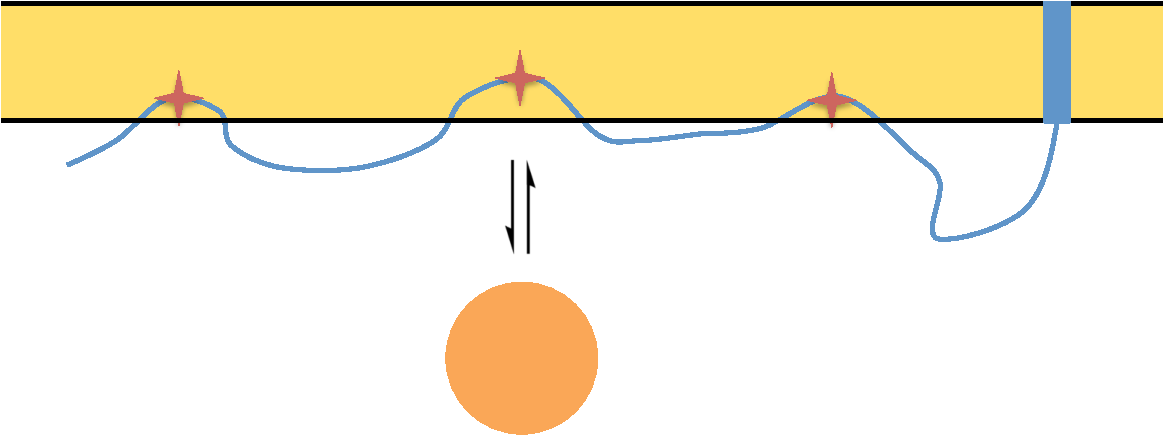
\includegraphics[width=0.7\linewidth]{ElectrostaticsDiagram.pdf}
    \caption{Cartoon of electrostatics model. FJC associates with membrane, burying modification sites within membrane rendering them inaccessible to ligands.\label{fig: ElectrostaticsCartoon}}
    \end{center}
\end{figure}


\subsubsection{Electrostatic Potentials}

The model where basic residues and tyrosines have similar energetics (Table \ref{table: BasicsYLocation}, Case 1) is the simplest case to explore. There are many types of electric potential we could explore for the correct behavior. Given that one of the phenomenons we wish to match is an approximately Gaussian distribution of both the tyrosines and polymer along the membrane edge, we use a parabolic-constant piecewise potential for our basic residues and tyrosines, instead of a Lennard-Jones potential. 

Parabolic-constant piecewise potential:

Piecewise potential (aka, parabola-constant), ($PC$):
\begin{equation}\label{eq: parabolaconstant}
E_{PC}(z_i) = 
\begin{cases}
k_{PC}z_i^2-E_0 	& z_i<\sqrt{\frac{E_0}{k_{PC}}}\\
0 & z_i \geq \sqrt{\frac{E_0}{k_{PC}}} \\
\end{cases}
\end{equation}

We have two possible potentials for the remaining amino acids. In general, the peptide should not be able to penetrate deep into the membrane. Therefore, we can implement a hardwall or softwall constraint. The hardwall will prevent the remaining amino acids from passing the beginning of the membrane. A softwall constraint will allow amino acids to enter the membrane, but will incur an energetic penalty. For this initial model, phosphotyrosines will follow this potential also.

Hardwall:

\begin{equation}\label{eq: hardwall}
E_H(z_j) = 
\begin{cases}
\infty 	& z_j < 0\\
0 & z_j \geq 0 \\
\end{cases}
\end{equation}


Softwall:

\begin{equation}\label{eq: softwall}
E_S(z_j) = 
\begin{cases}
k_Sz_j^2 	& z_j < 0\\
0 & z_j \geq 0 \\
\end{cases}
\end{equation}

We later develop a more complicated but possibly more motivated model with a repulsive force on the phosphotyrosines. There are many more basic residues compared to tyrosines in both the CD3$\zeta$ and $\epsilon$ chains. Therefore, in order to account for tyrosine phosphorylation being sufficient to dissociate the polymer from the membrane, we would expect a repulsive force from the phosphorylated tyrosines. We therefore shift future focus to models of Cases 3,4, and 5. We first consider the simple case where tyrosines do not experience their own potential but experience the potential of either the basic residues or experience the same potential as the rest of the amino acids. Since tyrosines are not positively charged, it seems less likely that they would experience the same force as the basic residues. Although their aromatic ring structure may help to anchor the polymer to the membrane once associated with the membrane, it would not drive the polymer to the membrane to begin with \cite{Lopez2015}. Therefore we focus future efforts on Case 5.

In this new model, we introduce a repulsive potential that acts only on the phosphotyrosines. We maintain the same potentials as above for the basic residues and the general amino acids, but now the tyrosines behave as generic amino acids. As our repulsive potential, we will include an exponential distribution where the repulsive effect of the membrane drops off quickly as the phosphotyrosines move further away from the membrane.

Exponential decay:

\begin{equation}\label{eq: exponential}
E_{\text{Repulse}}(z_i) = 
\begin{cases}
\infty	& z_i \leq 0\\
E_{R0}e^{-z_i/\bar{z}} & z_i > 0 \\
\end{cases}
\end{equation}


%%%%%%%%%%%%%%%%%%%%%%%%%%%%%%%%%%%%%%%%%%%%%%%%%%%%%%%%%%%%%%%%%%%%%%%%%%%%%%%%%%%%%%%%%%%%%%%%%%%%%
%%%%%%%%%%%%%%%%%%%%%%%%%%%%%%%%%%%%%%%%%%%%%%%%%%%%%%%%%%%%%%%%%%%%%%%%%%%%%%%%%%%%%%%%%%%%%%%%%%%%%
\subsection{Results}
\subsubsection{Model in which basic residues and tyrosines have similar energetics reveals puzzle in existing data}

We first explore the simplest model, where basic residues and tyrosines feel the same piecewise parabolic-constant potential and the phosphotyrosines feel the same softwall (or hardwall) potential as the rest of the residues (Table \ref{table: ElecPotentialRelationships}, Case 1). We first explore parameter space to find a set of parameters where the distribution of tyrosines is roughly gaussian centered at the membrane and extending about two Kuhn lengths in each direction (Condition 1). From this sweep, we see there are multiple parameter sets which achieve this distribution (Fig. \ref{fig: iSiteDistInitial}) For the following exploration of how phosphorylation impacts the distribution, we show the minimal parameters of those tested which give the desired distribution. Parameters which give reasonable distributions are: $k_{\rm{PC}}$ = 1 $k_BT/\delta^2$, $E_0$ = 10 $k_BT$, $k_S$ = 0.01 $k_BT/\delta^2$, where $\delta$ is the Kuhn length.


\begin{figure}[H]
\begin{center}
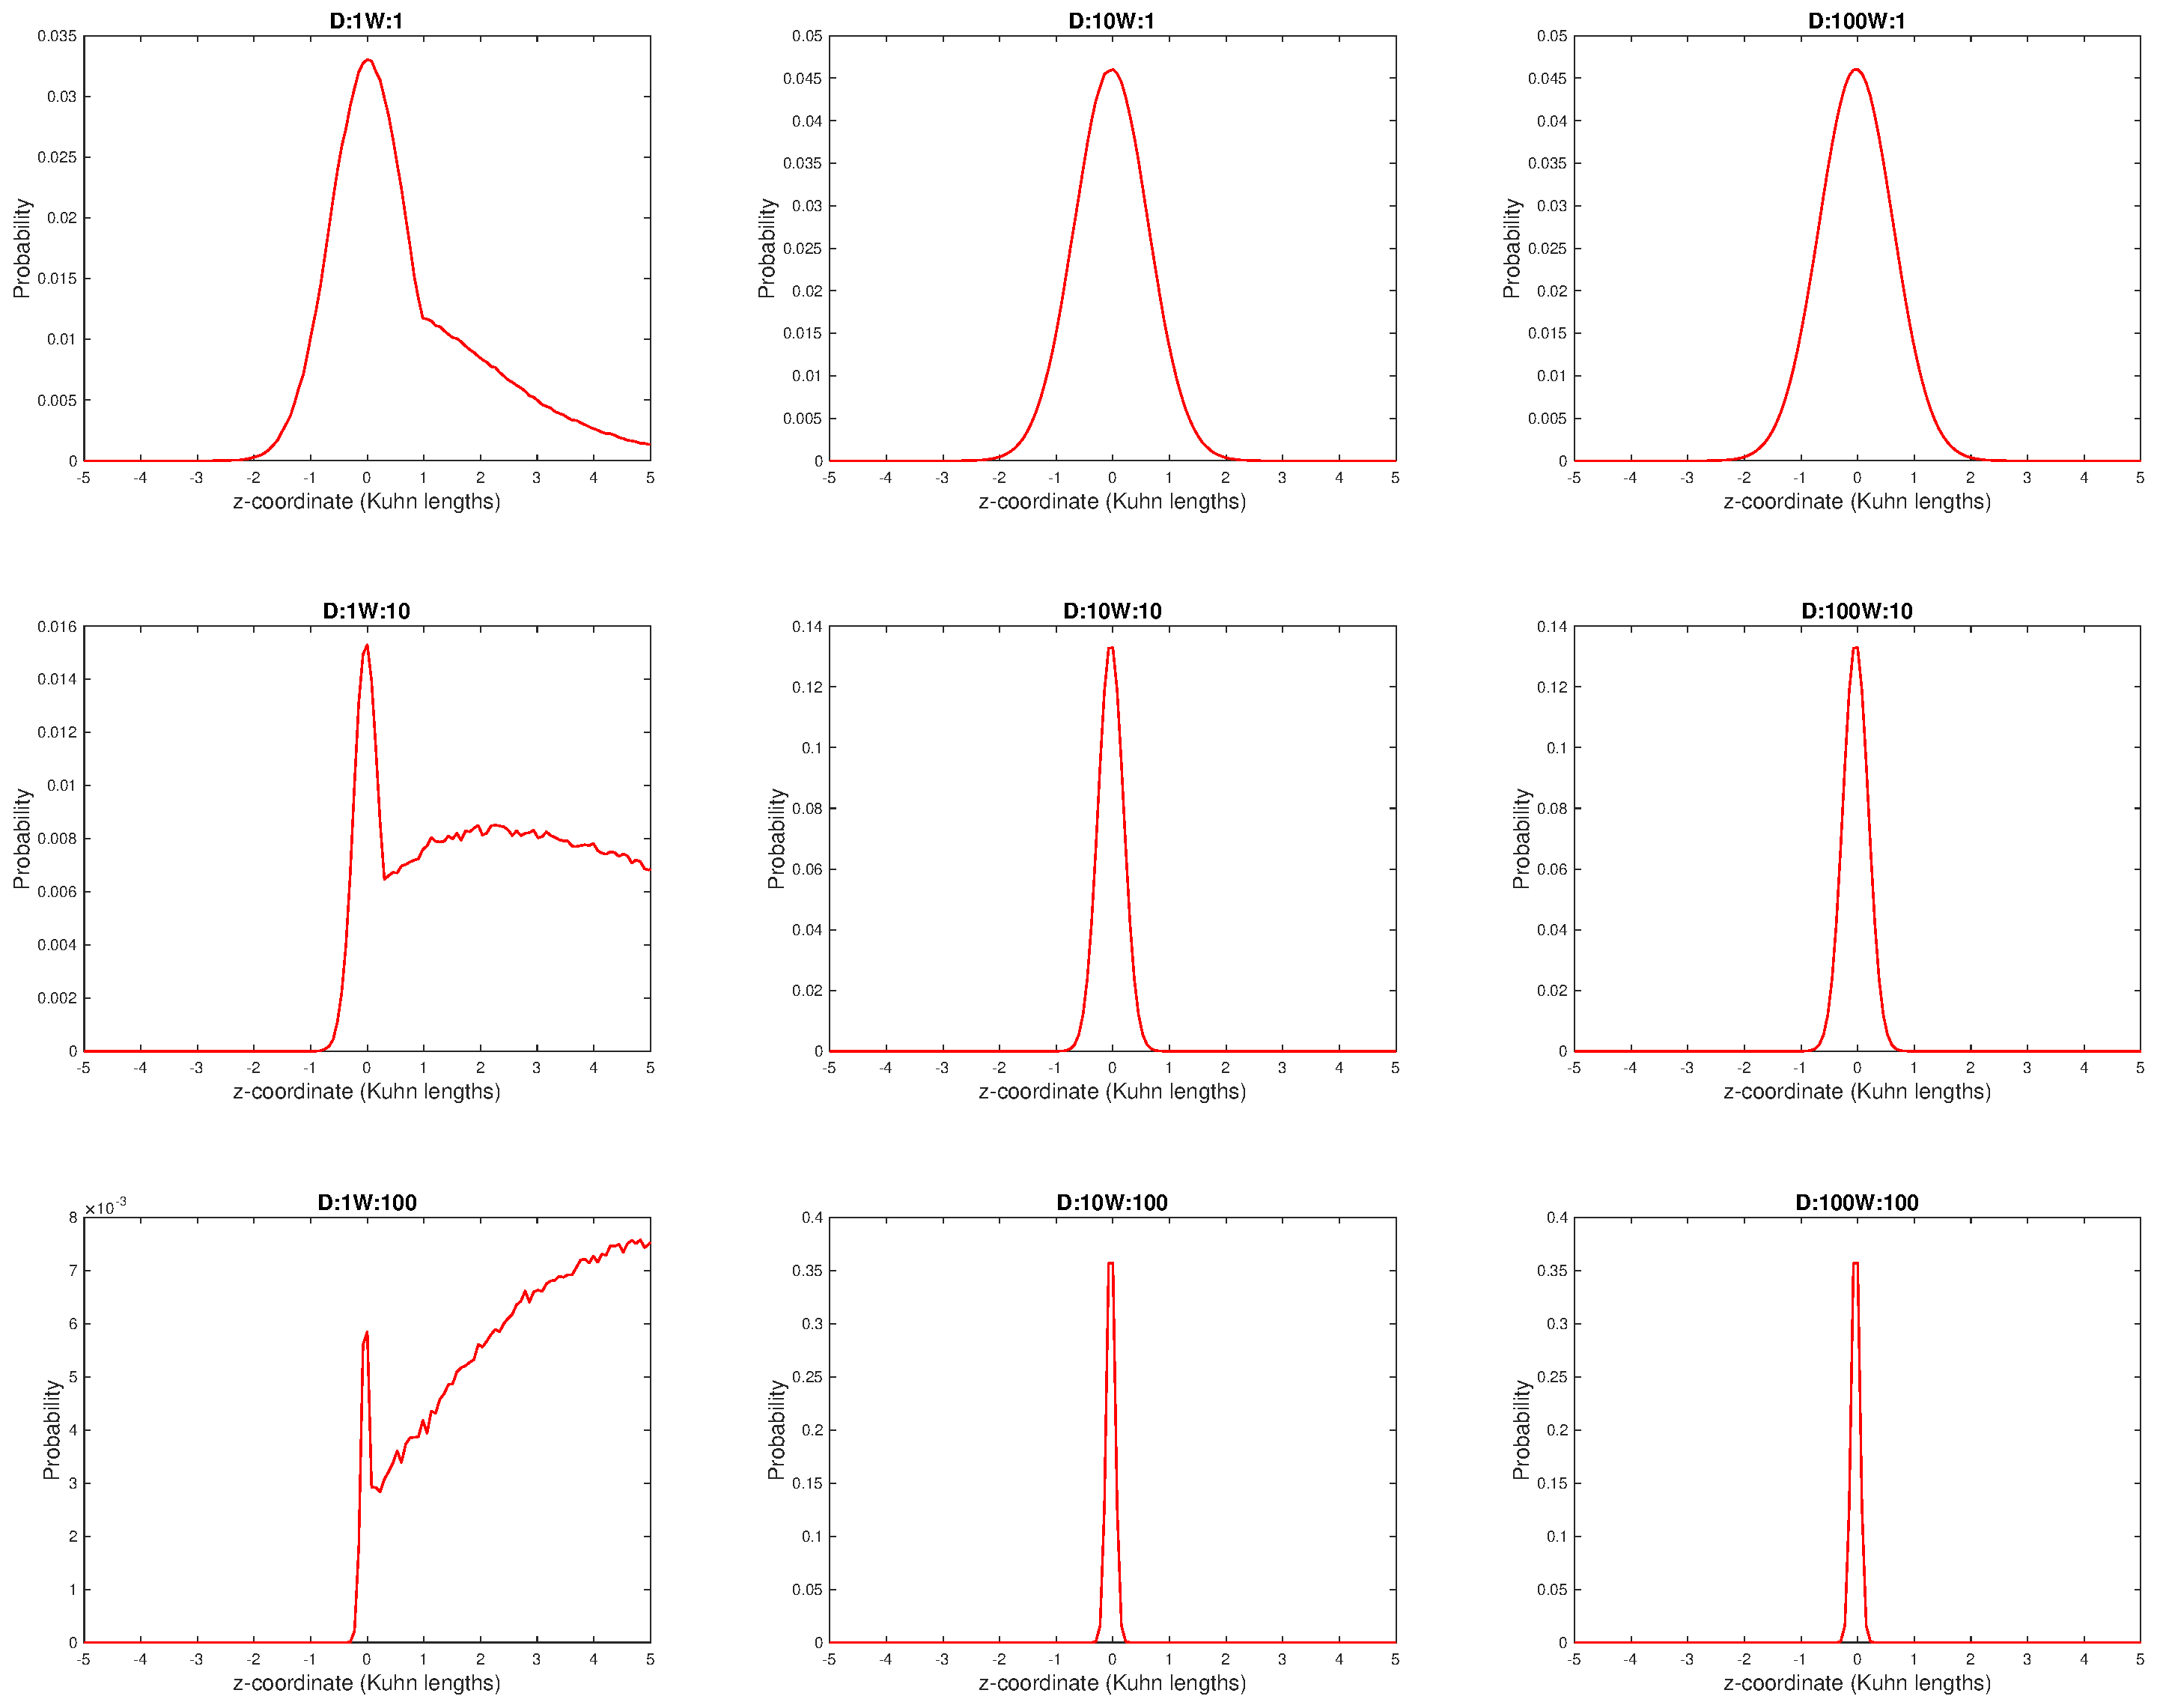
\includegraphics[width=0.8\linewidth]{ResultsFigures/CD3ZetaSoftwallPiecewiseBasicsY/DistributioniSite7.eps}
\end{center}
\caption{Polymer tip distribution resulting from parameter exploration of electric potentials. For this set, softwall potential width is set at 0.01. Both parabolic-constant potential depth and potential width range from $10^0$ to $10^{2}$.\label{fig: iSiteDistInitial}}
\end{figure}

We explore how phosphorylation, or removing tyrosines from the parabolic-constant potential and adding them to the softwall potential, impacts the distribution of the tyrosines and full chain. We find that under this regime, phosphorylating individual tyrosines does not impact the distribution of neighboring tyrosines (Fig. \ref{fig: Dist123456}). Additionally, phosphorylating two tyrosines does not influence the distribution of a tyrosines located between the two (Fig. \ref{fig: Dist135624}). We also find that even when all tyrosines are phosphorylated, the polymer does not fully dissociate from the membrane. This is represented by the distribution of the (basic) polymer tip residue distribution, which remains closely associated with the membrane. A non-basic, non-tyrosine residue located centrally is only slightly affected by the change in phosphorylation state. This result indicates these electric potentials may be insufficient to exhibit the characteristics displayed experimentally.

\begin{figure}[H]
\begin{center}
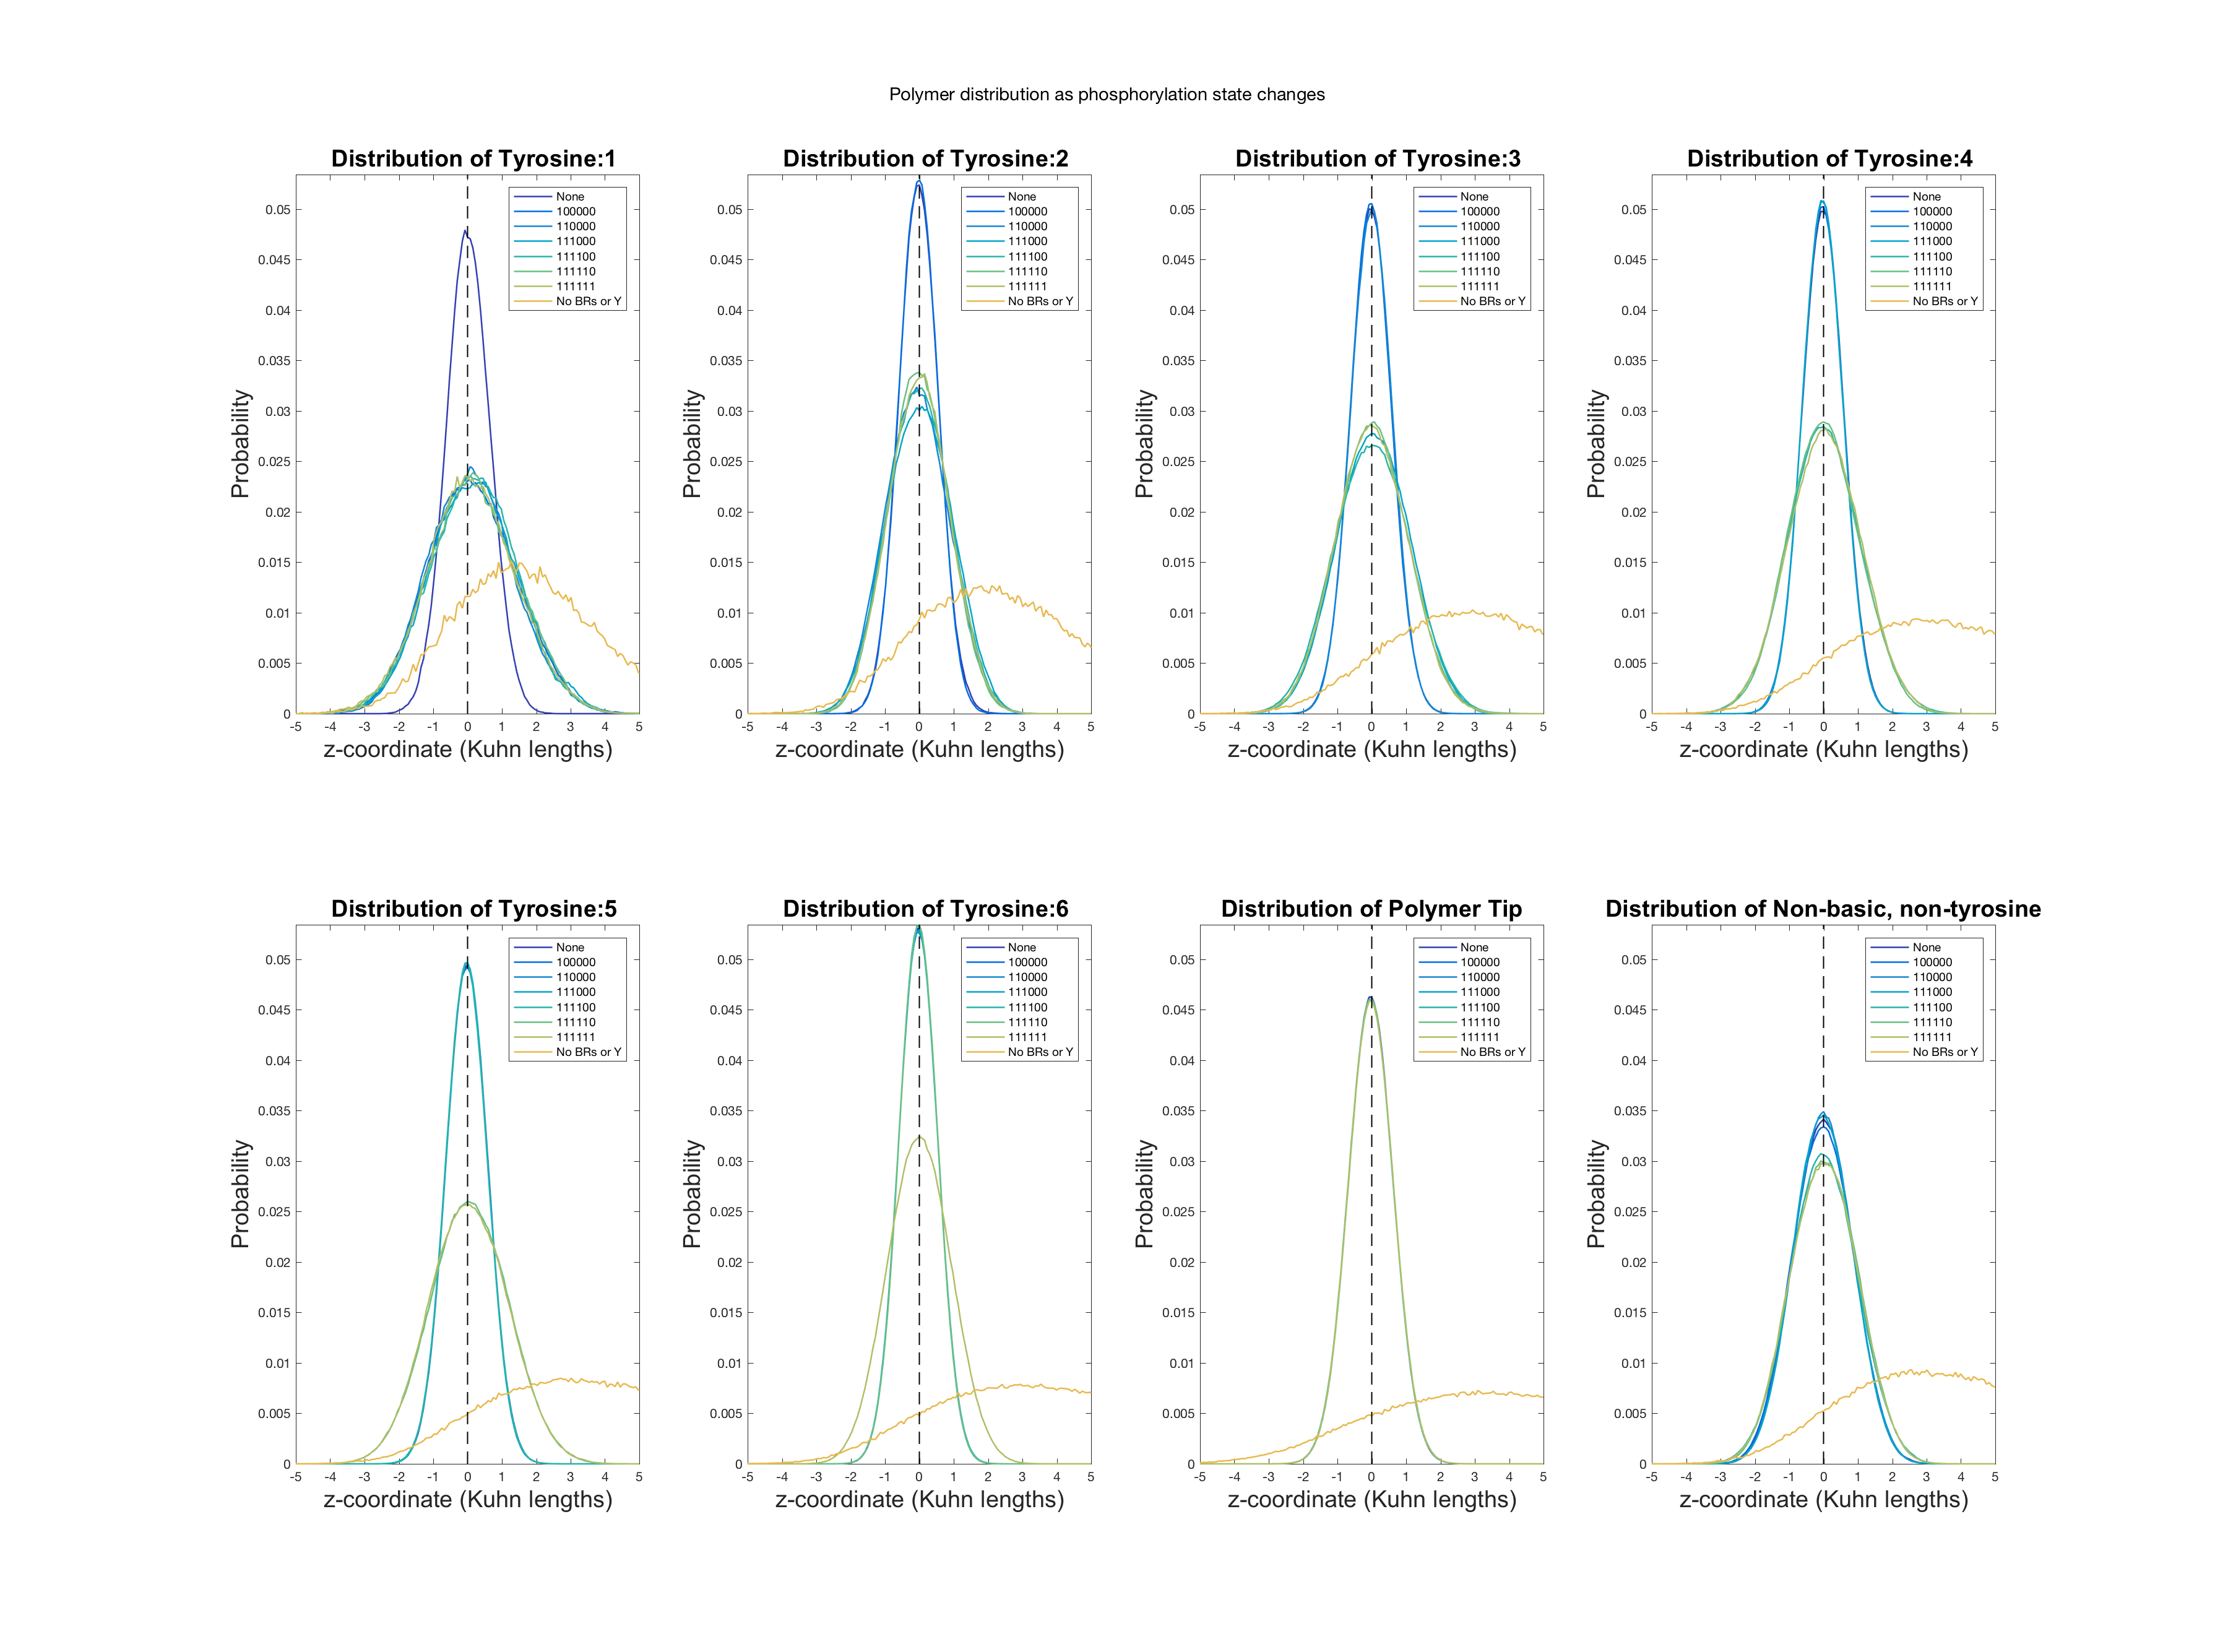
\includegraphics[width=\linewidth]{ResultsFigures/CD3ZetaSoftwallPiecewiseBasicsY/Phosphorylation/iSiteDistribution123456.eps}
\end{center}
\caption{Distribution of tyrosines, tail residue, and single non-basic residue for different phosphorylation states. Each curve has the phosphorylation state denoted as a series of 0's and 1's, with the tyrosines in order membrane-proximal to distal. Tyrosines are phosphorylated sequentially from proximal to distal. Tyrosines are indicated by 0, phosphotyrosines indicated by 1. Each distribution is plotted against the distribution created when all residues feel only the softwall potential. \label{fig: Dist123456}}
\end{figure}

\begin{figure}[H]
\begin{center}
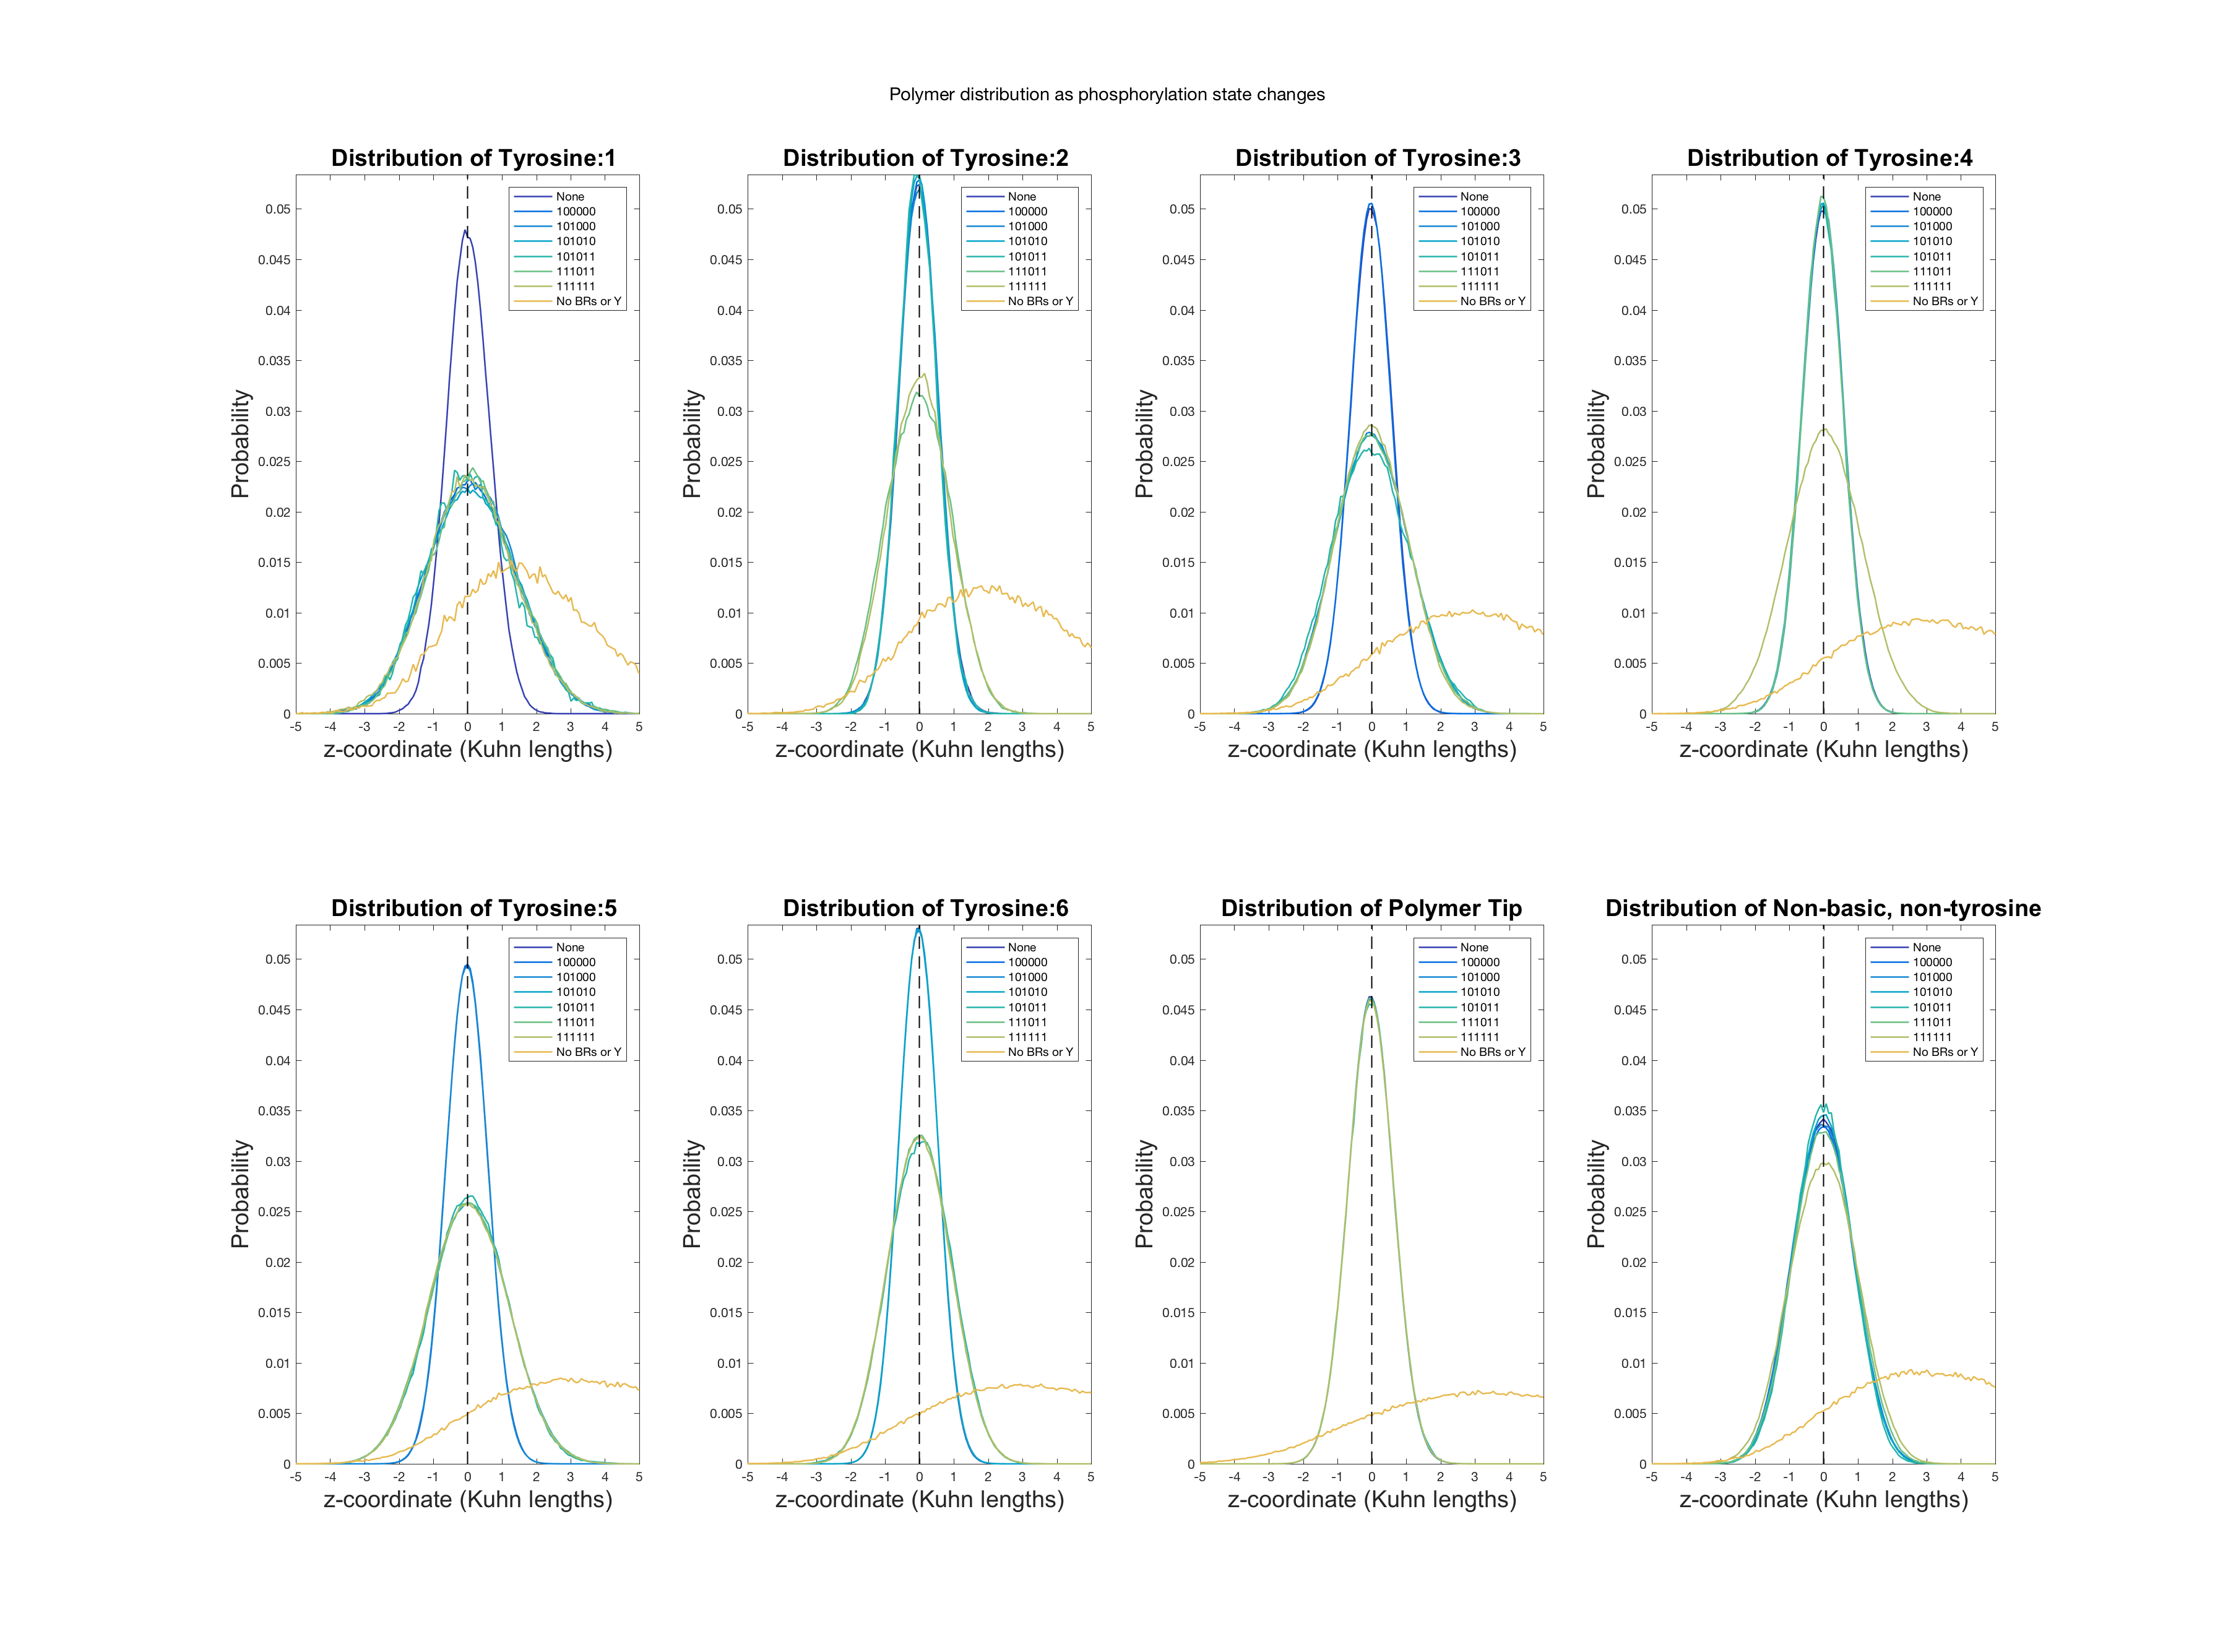
\includegraphics[width=\linewidth]{ResultsFigures/CD3ZetaSoftwallPiecewiseBasicsY/Phosphorylation/iSiteDistribution135624.eps}
\end{center}
\caption{Distribution of tyrosines, tail residue, and single non-basic residue for different phosphorylation states. Each curve has the phosphorylation state denoted as a series of 0's and 1's, with the tyrosines in order membrane-proximal to distal. Tyrosines are indicated by 0, phosphotyrosines indicated by 1. Phosphorylation sequence disordered to examine effect of two phosphorylation events on the distribution of an intermediate residue. Each distribution is plotted against the distribution created when all residues feel only the softwall potential. \label{fig: Dist135624}}
\end{figure}

\subsubsection{Initial parameter exploration of more general energetic model yields fit to polymer distribution}

We first want to match the distribution of the polymer to the molecular dynamics simulations from Lopez et al. We sweep through parameters for the basic residue potential and the softwall potential. The softwall potential permits a Gaussian curve for the tyrosine distributions. The hardwall condition (not shown) prevents the distributions from spreading below the zero axis where we have defined the membrane to be. When we explore these parameters, multiple possibilities for parameter sets emerge which meet the distribution conditions. Below are examples of distributions arising from our parameter exploration for both a tyrosine and a basic residue (Fig. \ref{fig: iSiteDist}, Fig. \ref{fig: tailDist}) We note that the tyrosines have a wider distribution than the basic residues since they do not directly feel the attractive potential. From these parameter sets, we may refine our parameter search and begin exploring how the distributions are affected when all tyrosines are phosphorylated. 

\begin{figure}[H]
	\begin{center}
		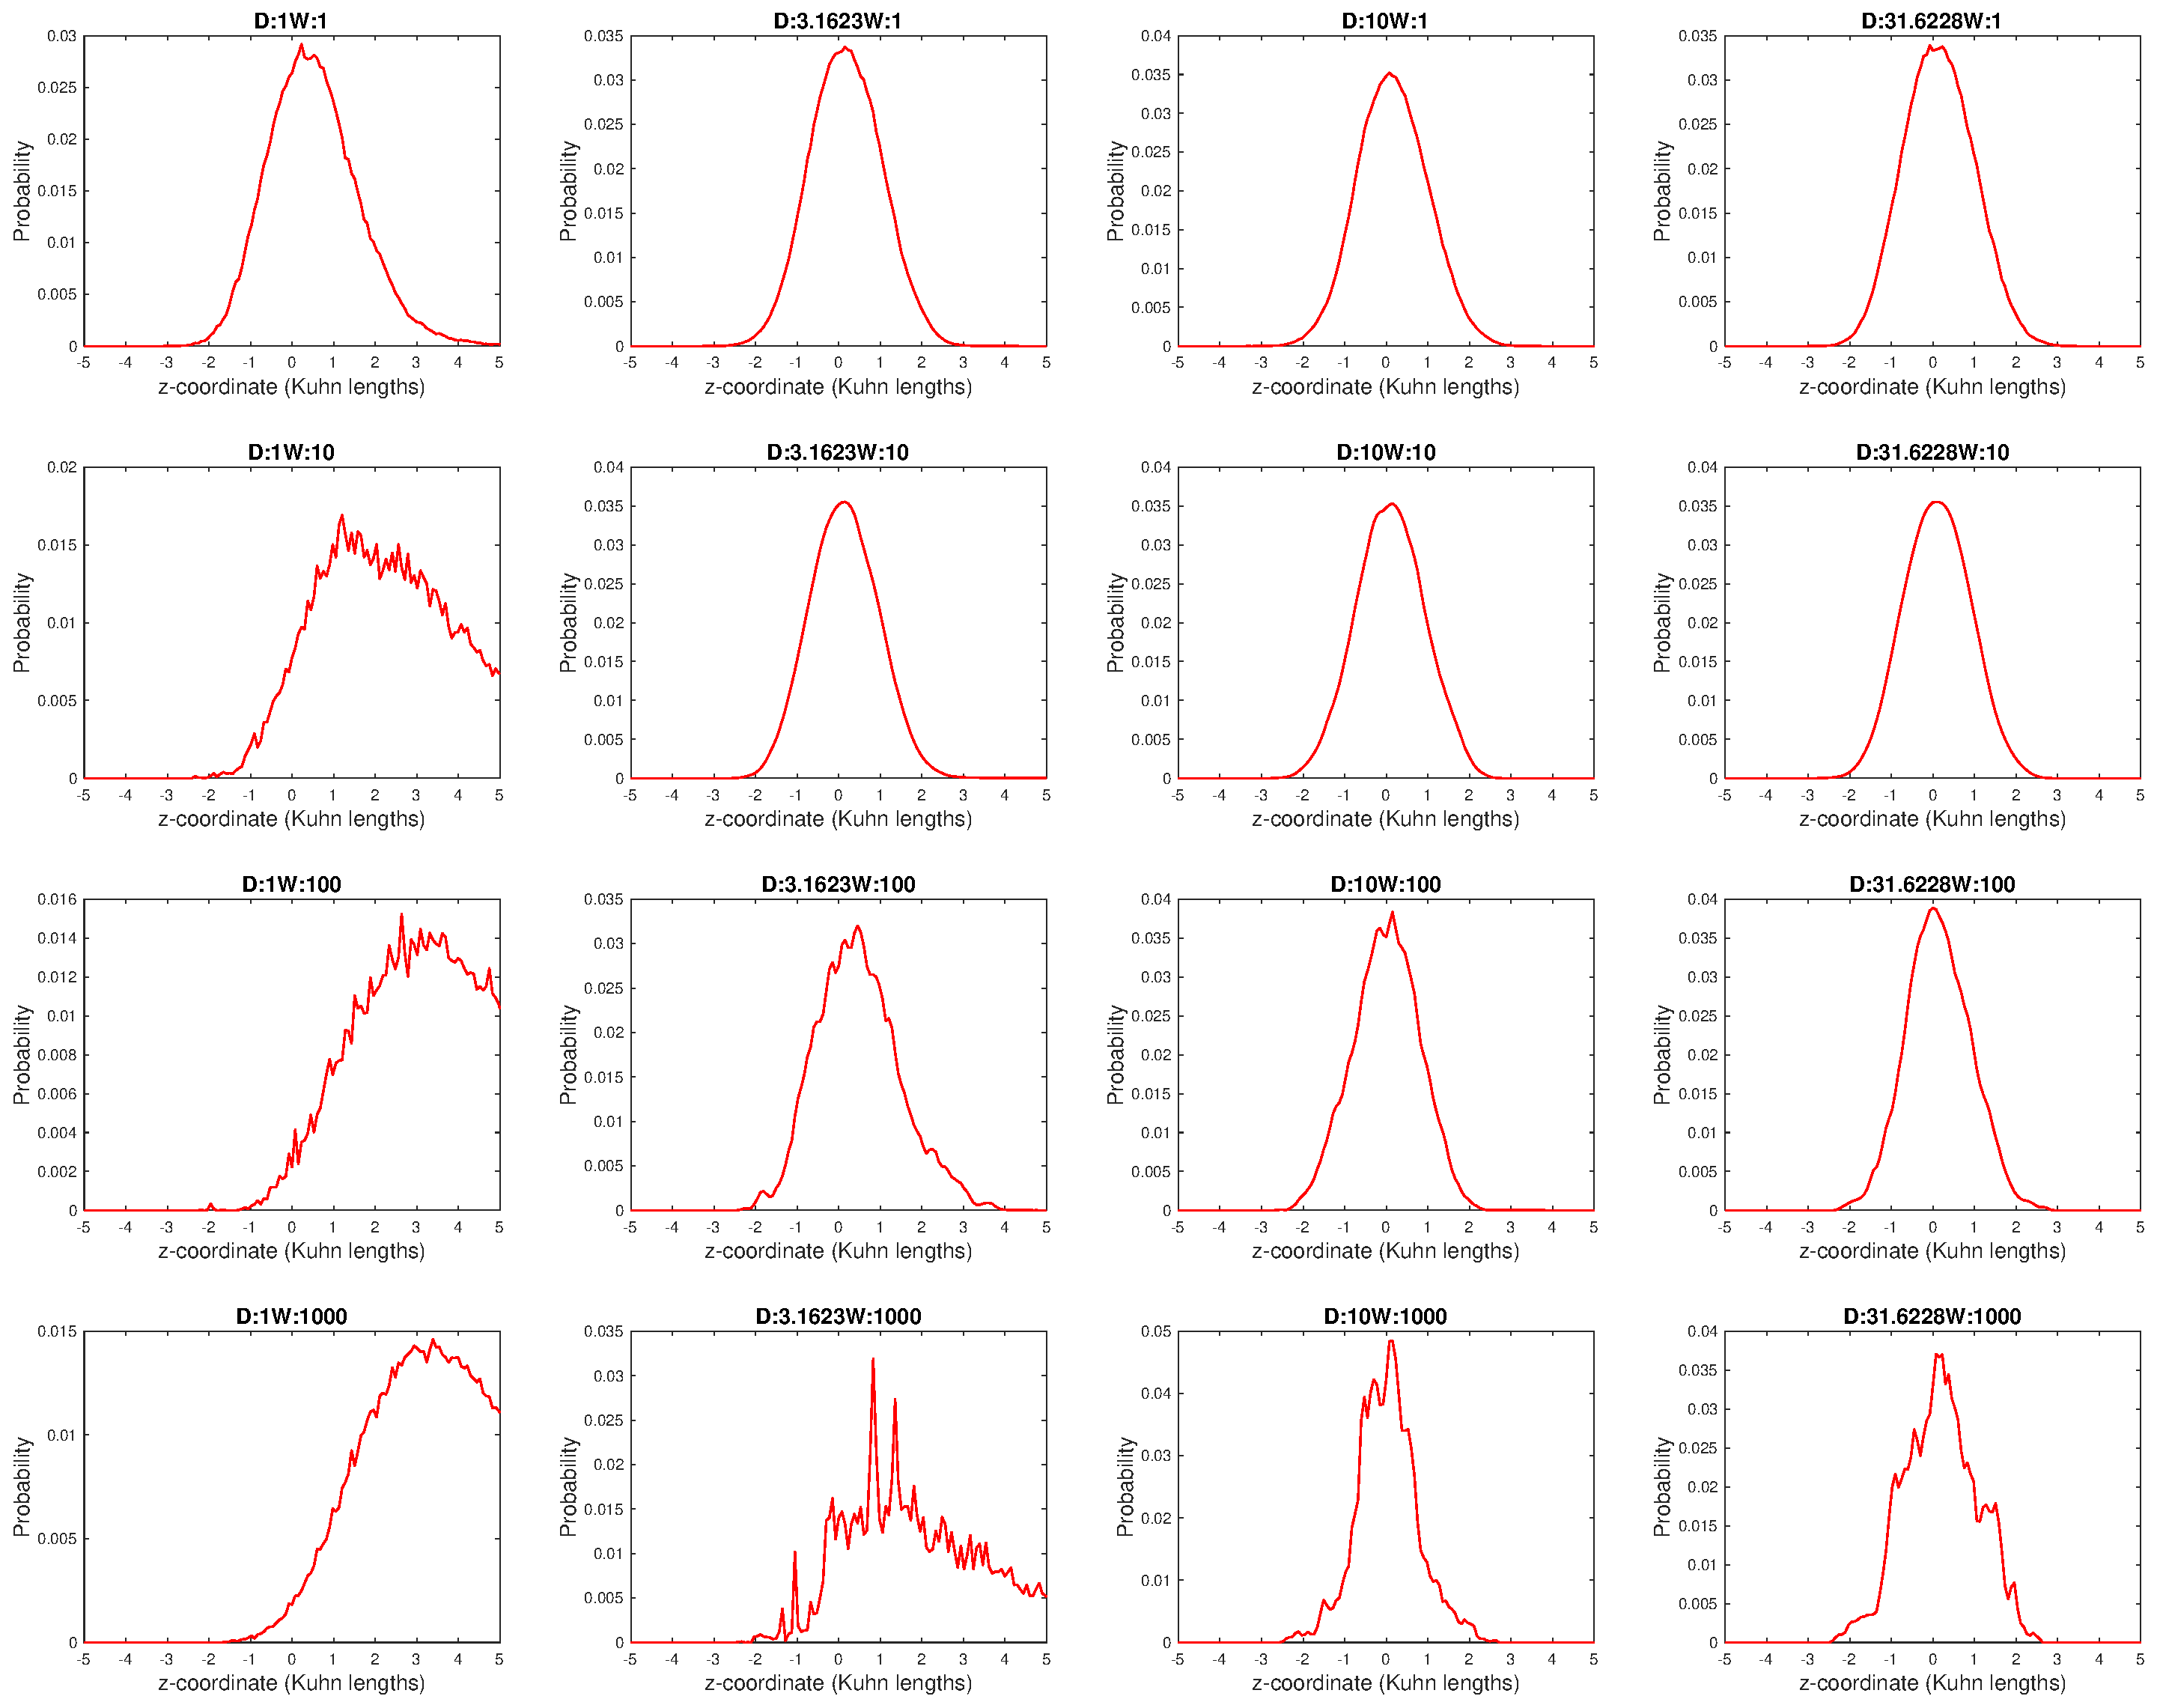
\includegraphics[width=0.8\linewidth]{ResultsFigures/Electro/DistributioniSite2.eps}
	\end{center}
	\caption{Tyrosine distribution resulting from parameter exploration of electric potentials. For this set, softwall potential is set at 0.1. Parabolic-constant potential depth ranges from $10^0$ to $10^{1.5}$, width ranges from $10^0$ to $10^3$.\label{fig: iSiteDist}}
\end{figure}

\begin{figure}[H]
	\begin{center}
		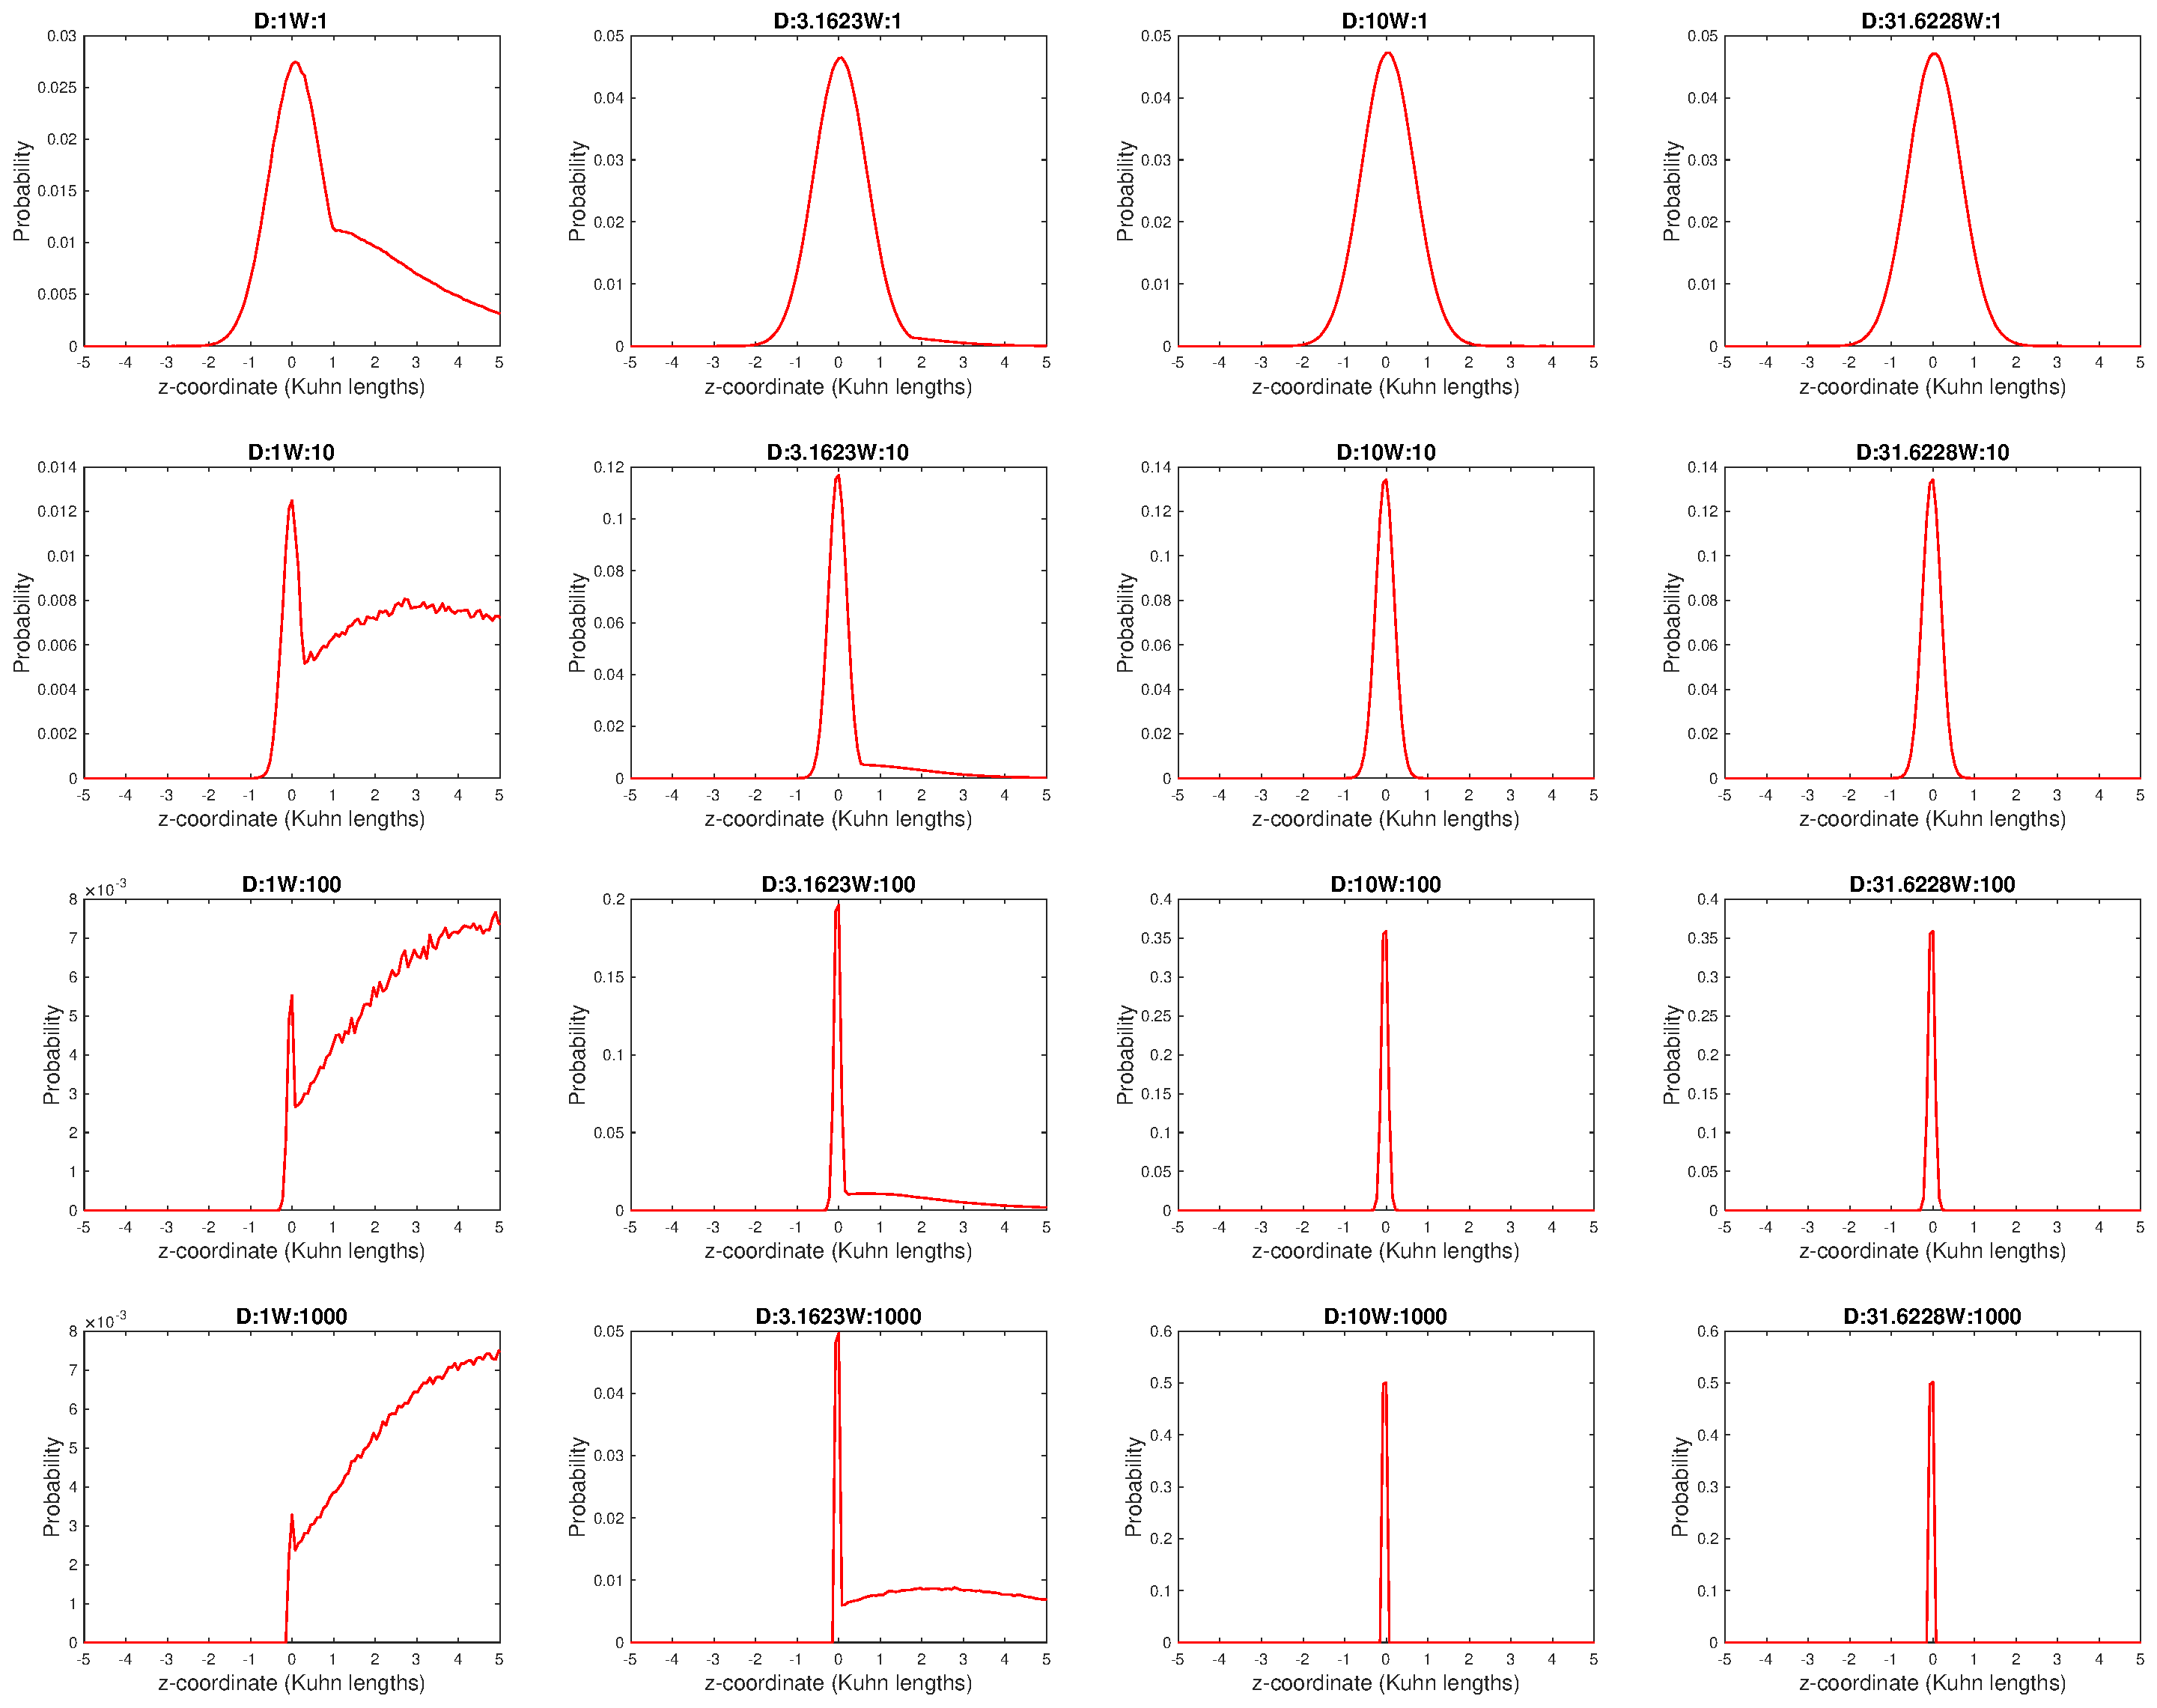
\includegraphics[width=0.8\linewidth]{ResultsFigures/Electro/DistributioniSite7.eps}. 
	\end{center}
	\caption{Polymer tip (basic residue) distribution resulting from parameter exploration of electric potentials. For this set, softwall potential is set at 0.1. Parabolic-constant potential depth ranges from $10^0$ to $10^{1.5}$, width ranges from $10^0$ to $10^3$.\label{fig: tailDist}}
\end{figure}




\subsubsection{Future Work: Parameter exploration}

First, we want to establish parameters (if they exist) which make our model exhibit the same behaviors as experimental and MD results. In particular, we now need parameters allowing the polymer to be free from the membrane when all tyrosines are phosphorylated. Either there will be only one reasonable parameter set which we can explore or there will be many parameter sets which display the desired properties. If there are multiple parameter sets then we may try to find other experimental results to narrow our parameter regime. Alternatively, we may explore two or three major parameter regimes: weakest, strongest, and median potentials. The results from a wide spread of parameters will give us an indication of how much the parameters matter to the qualitative results. 

Second, with our parameter sets, we will now explore the effect of phosphorylation on the accessibility of successive tyrosines to a kinase. We wish to see if there is a cooperative enhancement of the binding rates based on phosphorylation of previous residues. Cooperative phosphorylation could contribute to the first signaling event, explaining how an initial calcium release feeds back on the system, causing more CD3$\zeta$ chains to dissociate from the membrane and create a stronger signal \cite{Shi2013}.

Additionally, we will use this data to explore if there is a natural preferred binding sequence that arises. One would imagine that once a single tyrosine is phosphorylated then its nearest neighbor would be the most likely next target. However it is unclear if there is a first tyrosine that will be most likely to be phosphorylated and whether this will depend dominantly on basic residue distribution or on proximity to the transmembrane region. 

\subsubsection{Future Work: TCR clustering as cause of initial signal}
Independently or in conjunction with the above hypothesis, we formulate a second hypothesis to account for the initial dissociation from the membrane. When TCR triggering occurs, TCRs cluster \cite{Monks1998, Bunnell2002}. We hypothesize that a first chain will fall out of the membrane due to steric occlusion created by TCR clustering. With all six disordered subunits associated with the membrane, when the TCRs cluster, the subunits may become too crowded on the membrane and induce one or more to dissociate and become accessible to phosphorylation. We will explore how clustering of TCRs influences the association of the disordered subunits to the membrane. By modeling multiple disordered chains, we will estimate how many TCRs are needed and how tightly clustered they must be for a first chain to dissociate from the membrane and create the initial triggering event.

% potentially add image of mathematica plot to illustrate point


%%%%%%%%%%%%%%%%%%%%%%%%%%%%%%%%%%%%%%%%%%%%%%%%%%%%%%%%%%%%%%%%%%%%%%%%%%%%%%%%%%%%%%%%%%%%%%%%%%%%%
%%%%%%%%%%%%%%%%%%%%%%%%%%%%%%%%%%%%%%%%%%%%%%%%%%%%%%%%%%%%%%%%%%%%%%%%%%%%%%%%%%%%%%%%%%%%%%%%%%%%%
%\subsection{Discussion?}
%
%\hl{Maybe hybrid future work and discussion? or give if/then results sections?  (I.e. if we see coop, then this?)}
%
%Our initial model attempts show it is nontrivial to create a simple model where phosphotyrosines act to pull the rest of the polymer away from the membrane.























%%%%%%%%%%%%%%%%%%%%%%%%%%%%%%%%%%%%%%%%%%%%%%%%%%%
\end{document}
%%%%%%%%%%%%%%%%%%%%%%%%%%%%%%%%%%%%%%%%%%%%%%%%%%%





